\chapter{Methodology}\label{chap:chap4}

\section*{}



\section{Introduction}

According to the state of the art presented in chapter two, there are many means to, in some kind of automatic way, improve an applications performance. During my research, my focus was to find ways to automatically enhance the execution time in applications and programs. For this propose, Kremlin had a crucial impact in other to understand the viability of automatically parallelize code.

To study the utility and impact of automatic tools, the matrix multiplication algorithm will be used as a reference to make the performance comparison between original algorithm, an expert manually parallelizing the original algorithm and using the Kremlin's indications to parallelize the original algorithm.

To increase the credibility of this experiment, two similar algorithms for the matrix multiplication were used. As mentioned and explained in the chapter two, there is the traditional way of multiplying square matrices, naming as a quick reference \textit{Mult} algorithm, see in the appendix's list ~\ref{code:onmul} this algorithm implementation, written in C++ programming language; and the optimized algorithm that multiplies each element from the first matrix with the correspondent line of this matrix element but for the second matrix, naming this algorithm as \textit{MultLine}, see in the appendix's list ~\ref{code:onmuline} this algorithm implementation, written in C++ programming language. These algorithms differs from one another in the variables preparation and the order of the loops, which differs how the memory accessed. The \textit{MultLine} algorithm is an optimized version for matrix multiplication because it takes advantages of what is preloaded in cache and starts pre-calculating the intermediate values that will lead to the final and correct result of the multiplication, which means that won't be needed to load unnecessary values to cache memory and/or will need afterwards.  

Several experiments were conducted to understand the influence of Kremlin's indications versus code being manually parallelized  by an expert. The data's length, in this case, the matrix size; the number of threads used and if the code was parallelized were the used metrics to evaluate the results, based on a comparison of the execution time.

In this chapter it is explained the methodology and the steps followed to report in the Results and Discussion chapter the results and conclusions obtained from the performed experiences. This chapter also includes  detailed information of the acquired data from the conducted experiences, as in, how it is obtained and its meaning; also includes the methods that were used to analyse the obtained data and the reason behind those methods; and, in the end, how the data was validated in order to verify its correctness, accuracy and reliability.



\section{Research Method}

\begin{figure}[thb]
	\begin{center}
		\leavevmode
		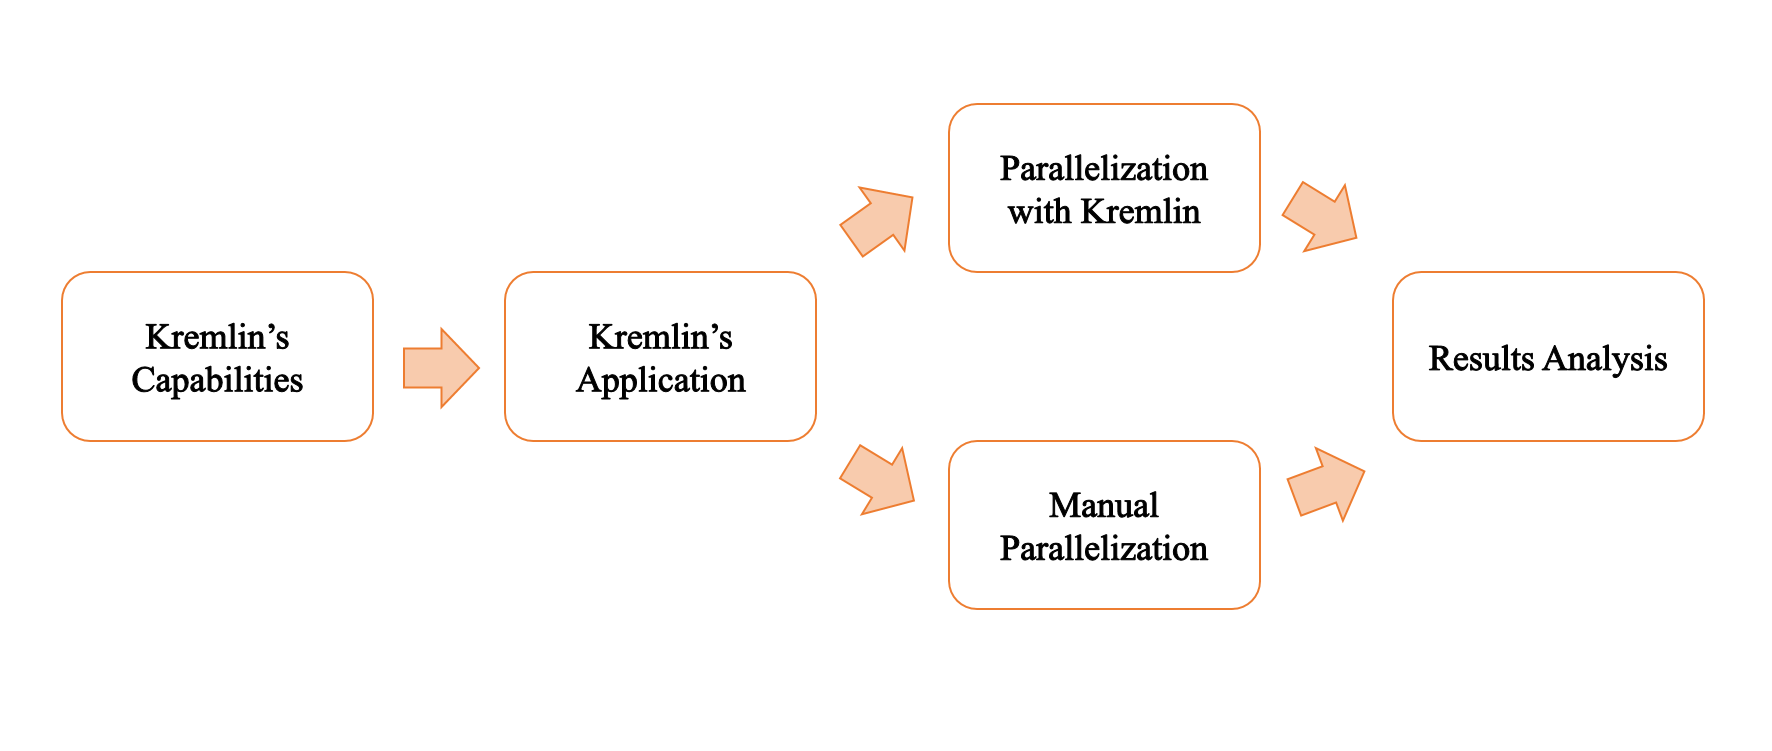
\includegraphics[width=1\textwidth]{methodology}
		\caption{Followed up methodology}
		\label{fig:workflow}
	\end{center}
\end{figure}


In Figure~\ref{fig:workflow} is outlined the steps that were followed to study the impact of the code being automaticaly parallelized. This methodology has five states. Firstly and using simple applications, an evaluation was made for Kremlin's tool in order to understand how to use this software tool and evaluate the results that it can achieve, for instance, if it has similar results comparing with an expert parallelizing manually the same code. After this, Kremlin will be applied to a set of codes with specific characteristics.

Before applying Kremlin, I manually parallelized the same sample of code in order to evaluate the results and, afterwards, compare with the Kremlin's output. Since these states (the experiences with Kremlin and the manual code parallelization) required several attempts there were transitions between these states. 

Finally, in the last state, after several attempts and tuning exercises applied to both code cases (Manual and Kremlin), data was collected from this experience to evaluate and validate its correctness in order to conclude how helpful can automatic parallelization can be.

To sum up, this methodology as three main stages: learn and evaluate  Kremlin's uses and results; finding the tuning parameter through several attempts using Kremlin's outputs and manually parallelize the application's code; and, in the end, compare and analyse the results in every attempt to take conclusions; 


\subsection{Deep learn on Kremlin's usage}

Firstly, and according to all tools/frameworks mentioned presented in the second chapter, \textit{Achieving the Highest Processing Power}, in the \textit{Using Code Parallelization} section ~\ref{sec:codeparallelization}, Kremlin was chosen because it presented the best results, easy usage and accessibility comparing to the others ~\ref{subsec:kremlin}.

Kremlin is a tool that indicates, for a sequential program, which block can be parallelised and some metrics theoretical calculated, such as, overall speedup; self parallelism for each block; the ideal time reduced for each block, in percentage; the actual time reduced for each block, in percentage; and the block coverage, in percentage. The way this tool was used is as it follows: first, an object file, \textit{*.o} extension, is required from the compilation of a sequential code. Afterwards, it is time to use the Kremlin's compiler with the generated object file so that it can profile the application. In order to do so, Kremlin's compiler runs the program as it is supposed to work. Now that the profiling is done, Kremlin generates the indications that should be followed to parallelize de provided sequential code. It also includes the blocks that can be parallelized and the impact of this theoretical parallelization with the calculations done during the profiling. Since this parallelization report is done, the developer has to interpret it, confront with the code an apply.

The Kremlin's usage seems easy, linear and fast forward, however it has some limitations that I experienced during the learning of Kremlin's capabilities: Kremlin's requires a specific environment mentioned in the Kremlin's repository ~\cite{KremlinRep}. It requires several software, libraries, compilers installations and a modern Unix operative system as its bases, such as MAC OS, RHEL 7 or other Linux distribution compatible with the software specification required. Additionally, when installing the Kremlin's tool, some minor fixes are required in order to successfully install.

From the experiences that I have been through, Kremlin has another limitation: it can not compile and profile all kind of programs: it can only profile programs that use C/C++ as its programming language; programs that take advantage of data structures from the \textit{Standard Library}, such as, stack, list, priority queue, queue, list, hash table, map, multimap, heap, and rest, since it doesn't recognize these structures; another Kremlin's limitations is its capability of compiling programs that have a deep function call level greater that seven. By deep function call level I mean the depth a function has starting from the \textit{main()} function until it is called, like a functions call tree. For instance: in a program there is the \textit{main()} function, a first level, that calls a \textit{foo1()} function, and this function calls a \textit{foo2()}, that this calls a \textit{foo3()} function, and so on. In this case, the depth of \textit{foo3()} function is four. Another small issue that Kremlin's tool has is the definition of the iterator variable used in the \textit{for}'s loops must be defined outside of the loop, as it is in C programming language.


\subsection{Kremlin's application in specific code samples}

After all the experiences made in the previous state and as mentioned in the introduction of this chapter, the matrix multiplication algorithm was used to see the potentialities of Kremlin's compiler to profile and identify the regions that can be parallelized. So, Kremlin was used in two similar, relatively similar in code structure, matrix multiplication codes. The reason behind the choice was because these two versions of the algorithm are really close to one another, which means that the testing environment is similar to one another, consequently, the results should be similar. 

\subsection{Code parallelization with Kremlin's data}

Kremlin's tool just points the regions/blocks where the program can be parallelized. In both code samples there are various numbers of inner \textit{for} loops, for the \textit{Mult} code  there are three inner \textit{for} loops, which one of them has a degree of three and the rest a degree of two; and for the \textit{MultLine} code there are four inner \textit{for} loops, which one of them has a degree of three and the rest a degree of two as well. At this time, after reading the report provided by Kremlin's tool, the developer must locate the loops, apply which loop should be parallelized, if it should be, and in case of inner \textit{for} loops, what loop should be parallelized using the OpenMP \textit{pragma} directives.

In my case, I followed all the instructions provided by Kremlin, located all the \textit{for} loops blocks indicated by kremlin's tool and applied the OpenMP \textit{pragma} directives. 

Following the two reports, ~\ref{report:onmulkremlin} ~\ref{report:onmulinekremlin}, and looking at the code's structure for both codes, it can be divided in 2 bigger parts: the \textit{for} loops used for matrices initialization and the \textit{for} loop for the matrix multiplication. With this information, understating the code and using an expert knowledge, the code parallelization was done.


\subsection{Manually Code parallelization}

In order to not be manipulated by the Kremlin's indications, the both codes were previously manually paralleliszd, this way it was guaranteed that the expert parallelization wasn't bias nor influenced.

For this parallelization, as mentioned before, it requires knowledge in, firstly, matrix multiplication algorithm; code understanding; best practice in what can and can not be parallelized, taking into account the overhead that could occur; and understand the thread behaviour in order to make it do the proper job without jeopardizing the programs outputs and/or performance.  

Analysing the code, only the \textit{for} loop for the matrix multiplication was parallelized and applied the OpenMP \textit{pragma} directives to the innermost \textit{for} loop. In this case, each code as a slight difference because for \textit{Mult} code each value of the result matrix must be calculated individually, so each thread is responsible for it and must treat that value as a private variable that isn't shared by the other threads. In the opposite, and since the \textit{MultLine} code calculates the values by adding the multiplication to the respective matrix's cell, each thread does not need to have their own private variable.

The bigger part of the code responsible for the matrices initialization wasn't parallelised, unlike in kremlin's case, because the gain would be noticeable on a large matrix size or it even could cause thread trampling, which could lead an overhead increase. 


\subsection{Results analysis}

To obtain the final execution time of each implementation (Original Matrix Multiplication ~\ref{code:onmul}, Original Matrix Multiplication by line ~\ref{code:onmuline}, Manual Matrix Multiplication by an expert ~\ref{code:onmulmanual}, Manual Matrix Multiplication by line by an expert ~\ref{code:onmulinemanual}, Kremlin Matrix Multiplication ~\ref{code:onmulkremlin} and Kremlin Matrix Multiplication by line~\ref{code:onmulinekremlin}), these six implementations suffered many modifications and tweaks since this process is a try-error until it is found the believed best parallelization. It is hardly possible to parallelize a whole program at the first try.

After compiling all these implementations and registering all the execution time for different matrix sizes and number of threads (not applied to the Original codes), this data was organized so it could be used to compare results and conclude about the performed experiences.

\section{Data collection from conducted experiences}

From all the developed work, the obtained data can be divided in two moments: Kremlin's indications reports and the execution times for the six code variations.

\subsection{Kremlin's indications reports} 

For the \textit{Mult} ~\ref{report:onmulkremlin} and \textit{MultLine} ~\ref{report:onmulinekremlin} codes were generated a report done by Kremlin. This report displays for each parallelizable block:

\begin{description}
	\item[Time reduced] percentage of time reduced if parallelization is implemented;
	\item[Ideal Time reduced] percentage of  ideal time reduced if parallelization is implemented;
	\item[Coverage] percentage of sequential execution time in a block;
	\item[Self Parallelism] amount of parallelism in a block;
	\item[Parallelism type] classification of the parallelizable block;
	\item[Loop location block] lines range of the parallelizable block;
	\item[Function location] function name of the parallelizable block, mentioning the line where the function is defined;
	\item[File location] file name of the parallelizable block, mentioning the line where the function is called;
\end{description}

The guidelines given by the report must be followed by the order it is suggested because the first detected block has the biggest impact in programs performance and should be parallelized first. The Coverage and Self Parallelism are metrics that indicates the speedup of the block, which, consequently, interferes with the time reduced. This block speedup must be equal or less then the overall program speedup, based on Amdahl's law, and can be calculated as it follows ~\cite{Saturnino}:

\begin{equation}
speedup \leq \frac{1}{(1- Coverage) - \frac{Coverage}{Self Paralelism}}
\end{equation}

\subsection{Execution times for the code variations}

After running the six implementations, the results can be divided in three major groups and each group has got the respective implementations of the \textit{Mult} and \textit{MultLine} algorithms. Each group has its own experimental environment,  with their own variables and their own meaning according to the given context.

\subsubsection{Original code}

The Original code only variable is the matrix size. This group is  a reference group to compare the results of the others groups and to quantify the impact of the others groups. The results of this group are the execution times running both matrix multiplications algorithm versions.

\subsubsection{Manual code parallelization}

The Manual code parallelization by an expert has as variables the matrix size and number of threads used for each run. This group's results are the execution times for both matrix multiplication algorithm versions. These results were used to confront with the following group in order to evaluate the improvement that a guided parallelizations, using Kremlin, can for an application.

\subsubsection{Kremlin's code parallelization}

Like the previous group, Kremlin's code parallelization indications use the same variables and provide the same type of the results. However, this group is responsible to define if it is advantageous to use software tools to help with code parallelization, in an automatic way.


\section{Data analysis method}

Analysing data is a very important stage because it is necessary to have correct conclusions. From the experiments made a lot of data as been generated and without a proper organization it is hard to understand the meaning, therefore, hard to take good conclusions from its analysis. There are three groups of code and in each group two different algorithms implementation. In order to make a correct analysis from the execution times for each situation and comparing with the others cases, the collected results were stored in tables along with the experimental related variables. Additionally, calculations were required, such as, difference between executed times between groups and algorithm implementation; ratio between these executed times; the percentage of the increase/decrease for these executed times; and the impact in the execution time that the others two groups have comparing with the Original code group. After these data manipulation, the best way to analyse all this generated and calculated data is by a dispersion plot. Using a dispersion plot, it transforms data into information visually understandable and easier to conclude because these plots display the variation of results according to the experimental environment variables.


\section{Data validation}

A considerable amount of data was generated and, more importantly, it is important that this data is scientific correct, or at least there is an explanation. In order to keep its fidelity, it is crucial to validate each and every piece of data. The first measure is to have a critical position every time by questioning if the obtained values makes sense when compared with theoretical, or expected or referenced value. In this current case, for instance, the Original group implementation is the reference, which means if the other groups have a lower execution time, or the data has some defect caused by some hardware component, or the implementation isn't good enough, or any other reason that can justify the data invalidation.

Criticism can not be the only measure because it could be luck and the gathered data happened to be correct. It is important consistency. To do so, the tests must be performed several times under the same circumstances and with a plausible and  considerable amount of values to find patterns. For this particular case  it is used a matrix size large enough, [1000,2000,3000,4000], and a wide range for the number of threads, [1,2,3,4,5,6,7,8]. For instance, if the matrix size was small, such as one hundred, the execution time would be so low and with so much error accumulated since the CPU executed fast enough that it couldn't count the time with precision. 

Finally, to make reasonable comparisons and analogies between results, the experience environments must have some connection in its variables or environment. Without a connection, the data as no meaning, therefore, it turns impossible to take conclusions. In the performed experiences, it was used the same algorithm, Matrix Multiplication, with small modifications in the implementations but with the same structure. Additionally, the environment variables were the same: number of threads and matrix size.

  

